%16/09 - Blanca Lizarbe
\chapter{Introducción al procesado de imágenes}
\section{Formación de imágenes}
Hay muchas formas de obtener una imagen, dependiendo de la fuente de energía (p. ej., fotones, ondas de radio, ultrasonido) y del sistema detector que la capture. Los tipos de imágenes se clasifican según si la formación es directa o indirecta, analógica (continua) o digital, y según el tipo de energía utilizada (radiación electromagnética, acústica, etc.).

Una forma de clasificarlas es en función del tipo de energía o radiación utilizada. La luz visible es una pequeña parte del espectro electromagnético. Las imágenes biomédicas pueden generarse utilizando otras partes de este espectro (rayos X, radiofrecuencia), así como otras formas de energía como ondas mecánicas (sonar, ultrasonido) o campos (magnéticos, eléctricos).

Aunque el grueso del curso sea el análisis y procesado de las imágenes, es importante saber de dónde vienen y su contexto.
\begin{itemize}
\item La \textbf{formación de imagen de rayos X} proviene de una fuente emisora. Estos rayos interaccionan con el tejido biológico (son atenuados principalmente por absorción y dispersión). La radiación que atraviesa el tejido incide sobre un detector (que históricamente era una placa fotográfica o de película, pero hoy son casi exclusivamente detectores digitales como placas de fósforo o detectores planos).
\item La \textbf{formación de una imagen de Resonancia Magnética (RM)} se basa en aplicar un campo magnético estático y fuerte (B0) al tejido, alineando los momentos magnéticos de los núcleos de hidrógeno. Se aplican pulsos de radiofrecuencia (RF) para excitar estos núcleos, que al relajarse emiten señales de RF. Esta señal se detecta con bobinas. Utilizando gradientes de campo magnético (que varían el campo de forma lineal en el espacio), se puede codificar espacialmente la señal y reconstruirla digitalmente para asignar diferentes intensidades de señal a cada voxel (elemento de volumen 3D) o píxel (2D).
\end{itemize}

\subsection{De analógico a digital}
Para convertir una imagen analógica (como una placa de rayos X o una fotografía) a digital se utiliza un dispositivo de digitalización, como un escáner o un detector digital directamente. Este proceso implica \textbf{muestrear (sampling)} la imagen, dividiendo el espacio en una matriz discreta de elementos (píxeles), y \textbf{cuantizar} la intensidad de luz en cada punto, asignándole un valor digital discreto.

La resolución espacial tiene que ver con el nivel de detalle discernible, determinado por el tamaño del píxel y las propiedades del sistema de imagen. Una imagen con muchos píxeles pequeños (alta resolución) permite visualizar detalles finos y bordes definidos. En cambio, una imagen de baja resolución tiene pocos píxeles grandes, lo que resulta en una pérdida de detalles y una apariencia pixelada o borrosa al ampliarla.

Las imágenes con las que se suele trabajar en diagnóstico por imagen suelen representarse en escala de grises. Esto significa que a cada píxel se le asigna una intensidad lumínica representada por un valor numérico. En el formato estándar de 8 bits, este valor va de 0 (negro) a 255 (blanco), permitiendo $2^8 = 256$ tonos de gris intermedios. La cantidad de bits utilizada para representar el valor de un píxel se denomina profundidad de bits (bit depth).
%Importante el concepto de 256 niveles de gris y los 8 bits

Cualquier sistema moderno de formación de imagen biomédica integra \textbf{sensores} (o detectores) y un \textbf{conversor de analógico a digital (ADC).} La imagen digital se debe guardar, procesar y, en ocasiones, se reconvierte a analógico (por ejemplo, mediante una pantalla) para su visualización.

\section{Procesado de imágenes digitales}
Dentro del procesamiento de imagen hay varias categorías o pasos:
\begin{enumerate}
\item \textbf{Mejora o Realce de la Imagen (Image Enhancement):} Técnicas para ajustar propiedades como el brillo, el contraste o para aplicar filtros (como la convolución) con el fin de hacer ciertas características más visibles para el observador humano o para un algoritmo posterior. Incluye la corrección de algunos artefactos.
\item \textbf{Restauración de Imagen (Image Restoration):} Su objetivo es eliminar o reducir la degradación (como el desenfoque o el ruido) utilizando un modelo de cómo se degradó la imagen. Se busca aproximarse a la imagen original no degradada.
\item \textbf{Análisis de la Imagen (Image Analysis):} Procesos como la segmentación (delimitación de regiones de interés), la extracción de características (cálculo de métricas cuantitativas) y la clasificación de objetos.
\item \textbf{Compresión de Imagen (Image Compression):} Técnicas para reducir el tamaño de los archivos de imagen para su almacenamiento o transmisión eficiente (p. ej., JPEG, JPEG 2000, DICOM con compresión).
\item \textbf{Síntesis de Imagen (Image Synthesis):} Generación de imágenes a partir de modelos o datos, como en la reconstrucción tomográfica o la generación de imágenes mediante Inteligencia Artificial.
\end{enumerate}

\subsection{Image enhancement}
Las imágenes biomédicas se utilizan para el diagnóstico, tanto \textbf{cualitativo} (observación visual de morfología) como \textbf{cuantitativo} (medición de parámetros fisiológicos o bioquímicos). Para el diagnóstico cualitativo, se tratan las imágenes para reducir ruido o realzar bordes. En las imágenes cuantitativas, el valor numérico del píxel tiene significado físico (p. ej., unidades Hounsfield en TC, concentración de un contraste, valores T1 o T2 en RM). Por ello, al manipular estas imágenes para su análisis, es crucial utilizar técnicas que no alteren o que corrijan de manera controlada los valores subyacentes, preservando la información biológico-física. A menudo, la consistencia en el procesamiento (aplicar el mismo algoritmo a todos los sujetos de un estudio) es más importante que la absolutez del valor.

Los \textbf{artefactos} son patrones o estructuras presentes en la imagen que no corresponden a la anatomía o fisiología real del sujeto, sino que son causados por el equipo, el protocolo de adquisición o el propio paciente. Estos incluyen desde artefactos por metal (implantes) hasta los causados por el movimiento voluntario o involuntario del paciente durante una adquisición, especialmente si es larga. La \textbf{reducción de ruido} (ruido aleatorio inherente a cualquier medición física) es también esencial para mejorar la relación señal-ruido (SNR).

Hoy día, las técnicas de \textbf{aprendizaje automático (machine learning),} y en particular las \textbf{redes neuronales convolucionales (CNN),} se utilizan extensamente. Un ejemplo es el entrenamiento de redes con pares de imágenes: una entrada degradada (p. ej., con artefactos de movimiento o ruido) y una salida objetivo de referencia ("ground truth") de alta calidad. La red aprende la transformación para mapear la imagen defectuosa a una versión corregida. Es importante destacar que a menudo el "ground truth" perfecto no existe \textit{in vivo}, por lo que los modelos se entrenan con datos simulados o con imágenes de alta calidad adquiridas en condiciones ideales.

Para corregir el ruido, una técnica común es el \textbf{filtrado espacial}. Un ejemplo básico es el \textbf{filtro Gaussiano}, que suaviza la imagen promediando los valores de los píxeles vecinos, ponderados por una función Gaussiana. Esto homogeniza las regiones y reduce el ruido, pero a costa de una potencial pérdida de detalle (suavizado de bordes). La operación se aplica deslizando un kernel (ventana) sobre la imagen, realizando una \textbf{convolución} (producto punto entre el kernel y los píxeles subyacentes) en cada posición.

\begin{figure}[h]
\centering
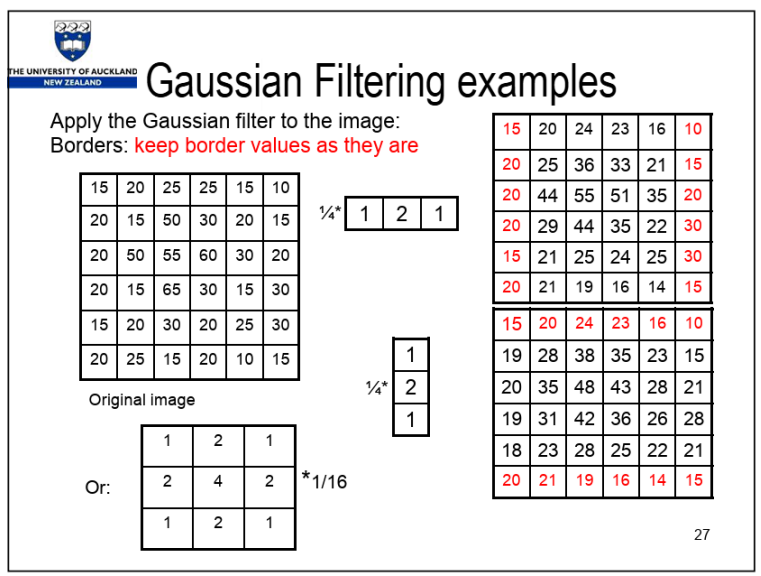
\includegraphics[width = 0.8\textwidth]{figs/gaussian-filter.png}
\caption{Ejemplo de filtro Gaussiano. Se aplica la matriz izquierda inferior sobre la imagen original, multiplicando los valores por la matriz de filtro y dividiendo por 16. Esto se realiza sobre cada píxel a excepción de los bordes. Por ejemplo, para el píxel con valor 15 de la segunda fila, segunda columna: $(15*1 + 20 * 2 + 25 * 1 + 20 * 2 + 15 * 4 + 50 * 2 + 20 * 1 + 50 * 2 + 55 * 1)/16 = 455/16 = 28,4375 \approx 28$, que es el valor del píxel de la matriz derecha inferior.}
\end{figure}

Mejora de la Resolución: El término general es superresolución (super-resolution). Este proceso busca estimar o reconstruir una imagen de alta resolución a partir de una o varias imágenes de baja resolución. El objetivo es recuperar detalles finos perdidos durante la adquisición, lo que conduce a una visualización más clara y puede facilitar un diagnóstico más preciso. Es importante distinguirlo de un simple zoom o interpolación, que agranda los píxeles sin añadir información nueva real. Las técnicas de superresolución pueden ser:
\begin{itemize}
\item \textbf{Basadas en reconstrucción:} Utilizan múltiples imágenes sub-píxel de la misma escena y algoritmos para fusionarlas.
\item \textbf{Basadas en aprendizaje:} Utilizan redes neuronales (como CNNs) entrenadas con pares de imágenes (baja/alta resolución) para aprender el mapeo que añade los detalles faltantes.
\end{itemize}

\subsection{Image analysis}
La \textbf{segmentación} es un paso fundamental en el análisis de imágenes. Su objetivo es dividir una imagen en regiones o estructuras significativas, permitiendo extraer y cuantificar la información de interés. Por ejemplo, aislar solo los huesos en una Tomografía Computarizada (TC), delimitar un tumor, o separar el ventrículo izquierdo en una imagen cardiaca.

Se lleva a cabo mediante algoritmos que identifican boundaries (bordes) o regiones homogéneas basándose en propiedades como la intensidad, el color, la textura o el contexto. No se limita solo a la extracción de bordes; existen múltiples enfoques:
\begin{itemize}
\item Basados en umbral (thresholding): Separan según el valor de intensidad.
\item Basados en regiones (region growing, watershed): Agrupan píxeles conectados con propiedades similares.
\item Basados en bordes (edge detection): Identifican discontinuidades en la intensidad (usando operadores como Sobel, Canny).
\item Basados en modelos (active contours, level sets): Utilizan curvas o superficies que evolucionan para ajustarse a los contornos.
\item Basados en aprendizaje (Machine/Deep Learning): Las redes neuronales (especialmente las U-Net) aprenden a segmentar a partir de ejemplos etiquetados.
\end{itemize}

El \textbf{registro de imágenes (Image Registration)} es el proceso de alinear geométricamente dos o más conjuntos de imágenes (datasets) adquiridas en diferentes momentos, desde diferentes modalidades o desde distintos puntos de vista. El objetivo es establecer una correspondencia punto a punto entre ellas para poder comparar, fusionar o analizar la información de forma coherente.

Esto se logra encontrando la transformación espacial óptima que mapea los puntos de una imagen (imagen móvil o "moving") sobre los de otra (imagen de referencia o "fixed"). Los tipos de transformación, ordenados de menor a mayor complejidad y flexibilidad, son:
\begin{itemize}
\item \textbf{Registro rígido (Rigid):} Alinea imágenes solo con rotaciones y traslaciones (desplazamientos) globales. Preserva las distancias y ángulos entre todos los puntos. Es útil para imágenes de la misma anatomía sin cambios internos (p. ej., cabeza en diferentes estudios de RM).
\item \textbf{Registro por similitud (Similarity):} Añade escalado isotrópico (mismo factor de escala en todos los ejes) a la transformación rígida. Preserva las formas y los ángulos, pero no las distancias absolutas.
\item \textbf{Registro afín (Affine):} Incluye cizallamiento (shearing) y escalado anisotrópico (diferente factor en cada eje), además de las transformaciones rígidas y de escalado. Las líneas paralelas siguen siéndolo después de la transformación, pero los ángulos pueden no conservarse. Es útil para corregir diferencias de adquisición o geometría entre modalidades.
\item \textbf{Registro no rígido o deformable (Non-rigid/Deformable):} Maneja deformaciones elásticas o fluidas complejas, localizadas y no lineales. Es esencial para compensar movimientos de órganos (como el corazón o los pulmones), cambios anatómicos (crecimiento de un tumor) o para alinear imágenes de pacientes diferentes en un atlas poblacional.
\end{itemize}
